\documentclass{controle}
\usepackage{main}

\title{Contrôle n°5 : Fonctions exponentielles}
\author{TSTMG1}
\date{Vendredi 17 Avril}

\begin{document}
\titleandname{}
\instructions[Autorisée]

\vspace*{0.5cm}

\begin{questions}
\titledquestion{Monotonie}[5] 

\begin{parts}
\part[3] Sans justifier, dire si chacune des fonctions suivantes est croissante ou décroissante :
\begin{subparts}
\subpart $x \mapsto 3 \times 5^x$
\subpart $x \mapsto -2 \times 4^x$
\subpart $x \mapsto 0,8 \times 0,75^x$
\subpart $x \mapsto -3,7 \times 0,34^x$
\subpart $x \mapsto -0,99 \times 1,001^x$
\subpart $x \mapsto 1,5 \times 1,8^x$
\end{subparts}
\part[2] On donne quatre fonctions exponentielles de la forme $x \mapsto a^x$ (on constate que $k = 1$) :
\begin{oneparchoices}
\choice $f : x \mapsto 2^x$
\choice $g : x \mapsto 1,5^x$
\choice $h : x \mapsto 0,75^x$
\choice $j : x \mapsto 0,40^x$
\end{oneparchoices}
On représente les courbes représentatives de ces quatres fonctions sans les nommer. Associer à chacune de ces courbes la fonction correspondante.

\vspace*{0.5cm}

\begin{center}
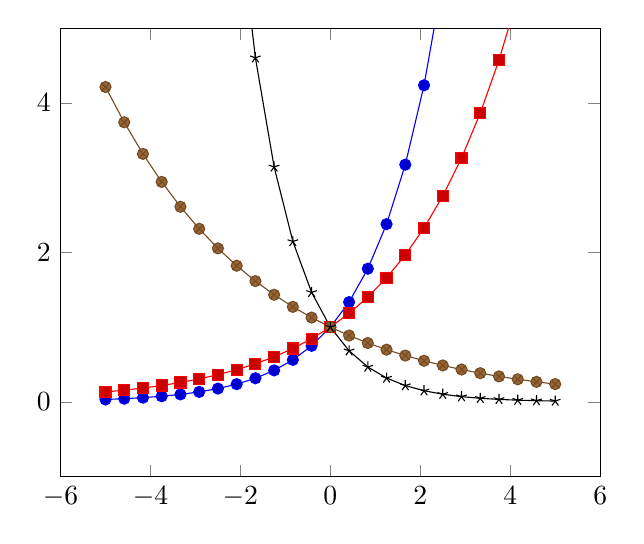
\begin{tikzpicture}
\begin{axis}[ymin=-1,ymax=5]
\addplot {2^x};
\addplot {1.5^x};
\addplot {0.75^x};
\addplot {0.4^x};
\end{axis}
\end{tikzpicture}
\end{center}
\end{parts}

\newpage

\titledquestion{Algèbre}[5]
\begin{parts}
\part[3] Simplifier les expressions suivantes pour qu'elles soient de la forme $a^p$.
\begin{subparts}
\subpart $a^{12} \times (a^4)^5$
\subpart $\dfrac{a^{1,9} \times a^{3,6}}{a^{2,3}}$
\subpart $\dfrac{(a^6)^0,5}{(a^{12})^{0,25}}$
\end{subparts}
\part[2] Résoudre dans $\R$ les équations suivantes :
\begin{subparts}
\subpart $x^2 = 5$
\subpart $x^5 = 2$
\end{subparts}
\end{parts}


\vspace*{0.5cm}


\titledquestion{Bénéfices/Risques}[8]
Une compagnie d'assurances s'intéresse à la tendance générale des accidents domestiques. Elle débute son étude en 2025 et constate que chaque année, la nombre d'accidents augmente de $7\%$. 
\begin{parts}
\part[1] Si on pose $(u_n)$ la suite donnant le nombre d'accidents à l'année $2025 + n$, justifier en une phrase que $(u_n)$ est une suite géométrique dont on précisera la raison.

\vspace*{0.5cm}

La compagnie utilise plutôt le modèle exponentiel pour représenter le nombre d'accidents de voitures par année. Elle obtient que la quantité $a(x) = 1000 \times 0,93^x$ représente le nombre d'accidents de voiture, où $x$ est le nombre d'années écoulées depuis le 1er Janvier 2025.

\part[1] Quelle valeur de $x$ permet de calculer le nombre d'accidents recensés le 1er Janvier 2025 ? Donner ce nombre.
\part[1] Même question pour le 1er Janvier 2027.
\part[1] Même question pour le 1er Juin 2030.

\vspace*{0.5cm}

La compagnie souhaite établir un modèle similaire pour les accidents du travail. Pour cela, on dispose d'un tableau recensant l'augmentation ou la diminution en pourcentages du nombre d'accident du travail tous les 5 ans pendant 15 ans :
\begin{equation*}
\begin{tblr}{hlines, vlines}
\text{Années écoulées : } & 0 & 5 & 10 & 15\\
\text{Évolution en \% : } & 0 & +12\% & -2\% & + 20\%\\
\end{tblr}
\end{equation*}

\part[2] En ne considérant que l'augmentation de $+12\%$ lors des cinq premières années, calculer le taux d'évolution moyen par année.
\part[2] En considérant l'évolution globale sur les quinze années, calculer le taux d'évolution moyen par année.
\end{parts}


\end{questions}
\end{document}